\documentclass{article}
\usepackage{indentfirst}
\usepackage{graphicx} % Required for inserting images

\title{Creating a Maritime Weather Forecast Model Using NOAA Buoy Climate Measurements}
\author{Austin Paczkowski}
\date{\today}

\begin{document}

\maketitle

\section{Introduction}

Oceans have played an integral part in human history for thousands of years. From using it as a method of transportation, transporting goods, and collecting seafood, humans depend on the ocean for survival. At the same time, maritime activities have caused countless fatalities due to the rather unpredictable and extreme weather conditions involved. As such, this human-ocean relationship creates a necessity to predict future weather phenomena, birthing the field of meteorology. By applying statistical methods and regression models to meteorological theory, it is possible to forecast weather conditions such as air temperature, sky clarity, precipitation, air pressure, wave height, and countless other factors to increase confidence in maritime navigation, thereby reducing fatalities. In this paper, we will transform a collection of ocean weather measurements, create a linear model-based weather forecast using this data, perform simulations with this weather forecast, and discuss avenues for further exploration as well as ideas for improvement.

\section{Transforming the Data}

\subsection{Introducing Buoy Data}

To begin, we will introduce our data \textit{marine-sample}, a collection of $n = 55$  weather measurements of buoy D5GN6 from the National Oceanic and Atmospheric Administration (NOAA) between January 12th and January 31st 2015\cite{noaaDatasetsClimate}. Of the 55 observations listed, each one contains 33 variables with various types of data. Each observation stores ID, time, and coordinates of the observation. In addition, each observation stores categorical and numerical variables providing information about ice, air pressure, temperatures, wave measurements, swell measurements, cloud coverage, visibility, precipitation, and wind. While the data may be dense with information, it is messy and primitive. As such, we need to transform the data into a useful and intuitive form for analysis and modeling.

\subsection{Cleaning the Data}

Upon viewing the \textit{marine-sample} data, each variable is recorded in one of two ways: as numerical values for objective measurements and as categorical letters or integers. Fortunately, there is a documentation file included with the data at NOAA \cite{noaaDatasetsClimate} that explains the meaning of the values in each column as well as the corresponding WMO Table Code \cite{WMOCodes2017} to use when necessary. As such, we will use these to interpret, understand, and transform the data for analysis and modeling.

\subsubsection*{Removing Useless Columns}

Nine of the 33 variables contain \texttt{NA} values for each observation. These include Ice Accretion, Thickness of Ice Accretion, Rate of Ice Accretion, Wet Bulb Temperature, Sea Temperature, Wave Direction, Low Cloud Type, Cloud Height Indicator, and Visibility Indicator. In addition, both Identification and Pressure Tendency have zero variability in their observations (all of them are the same). As such, we will remove these 11 columns, leaving us with 22 variables.

\subsubsection*{Latitude and Longitude}

The Latitude and Longitude columns contain coordinates from (0,0) where negative values are South and West respectively. As such, these values are stored as desired and require no transformation.

\subsubsection*{Timestamp}

The timestamps of the observations are stored as \texttt{YYYY-MM-DDThh:mm:ss}. Due to the sparsity and time frame of collected observations, only hour and day values are of any use for analysis. As such, we parse the timestamp into an hour column with the numeric \texttt{hh} value, a day column with the numeric \texttt{DD} value, and remove the timestamp column from our data.

\subsubsection*{Air Pressure}

There are two columns involved with air pressure: Sea Level Pressure and Characteristics of Pressure Tendency. We will transform Sea Level Pressure into millibars from inches of Mercury by multiplying each value by 33.8639. Upon viewing WMO Table 0200 \cite{WMOCodes2017}, there are 9 different classifications for the pressure. As such, we will transform these 9 classes into two major groups: Increasing Air Pressure and Decreasing Air Pressure.

\subsubsection*{Temperature}

There are two columns involved with temperature: Air Temperature and Dew Point Temperature. For both Air and Dew Point temperatures, the values are initially in Fahrenheit. As such, we will subtract by 32 and then multiply by $\frac{5}{9}$ to get the Celsius value of each observation.

\subsubsection*{Wave Measurements}

There are two columns involved with wave measurements: Wave Period and Wave Height. The Wave Period measurement is a categorical variable corresponding to a range based on WMO Table D5a \cite{WMOCodes2017}. For simplicity, we will record each observation as the mean value of these ranges and omit observations without a valid range. Wave Height is recorded as how many half meters high the waves are. As such, we will multiply these values by 0.5 to get the full meter values.

\subsubsection*{Swell Measurements}

There are three columns involved with swell measurements: Swell Direction, Period, and Wave Height. Swell Direction is a numerical measurement of how many degrees clockwise north the swell is traveling divided by 10. As such, we will multiply each value by 10 to get the full degree values. There is also 1 outlier of 380 degrees that will be removed. The Swell Period is recorded as is in seconds and requires no transformation. Swell Height is also recorded as how many half meters high the swells are. As such, we once again multiply by 0.5 to get the full meter values.

\subsubsection*{Cloud Measurements and Classifications}

There are six columns involved in classifying and measuring clouds: Total Cloud Amount, Low Cloud Amount, Cloud Height, Visibility, Middle Cloud Type, and High Cloud Type. Viewing WMO Table 2700 \cite{WMOCodes2017} for Total Cloud Amount and Low Cloud Amount, the values correspond to how many oktas the sky is covered in clouds. Because an okta is $\frac{1}{8}$ of the sky, we multiply each value by 0.125 to get a proportion for sky coverage for these variables. For Cloud Height, we assign each class to the corresponding mean value in the range given by WMO Table 1600 \cite{WMOCodes2017} to get numerical representations. We omit class 9 and A observations as they are not numerically representable. For Visibility, there are 10 classifications from WMO Table 4377 \cite{WMOCodes2017}. However, only classes 97 and 98 appear in our data. As such, we will transform these into their corresponding kilometer values 10 and 20 respectively. For the Middle Cloud Type, there are 11 classifications from WMO Table 0515 \cite{WMOCodes2017}. As such, we will simplify this to 3 classes by omitting class A and blank observations, assigning class 0 observations to \texttt{No Middle Clouds}, classes 1 and 2 observations to \texttt{Altostratus or Nimbostratus}, and classes 3, 6, 7, and 8 to \texttt{Altocumulus}. For the High Cloud Type, there are also 11 classifications from the sister table of WMO Table 0509 \cite{WMOCodes2017}. As such, we will again simplify this to 3 classes by omitting class A and blank observations, assigning class 0 observations to \texttt{No High Clouds}, classes 1 and 4 observations to \texttt{Cirrus}, and classes 5 and 8 to \texttt{Cirrostratus+}.

\subsubsection*{Weather}

There are two columns involved in classifying weather: Present Weather and Past Weather. Present Weather uses WMO Table 4677 \cite{WMOCodes2017}, involving 100 unique weather classifications. However, only a handful of them are used in our observations. As such, we will simplify this to 3 classes where we assign classes 1, 2, 3, and 13 to \texttt{No Precipitation}, class 80 to \texttt{Light Precipitation}, and classes 62, 82, 90, and 92 to \texttt{Moderate to Heavy Precipitation}. In addition, we will create an additional column called Present Weather Numeric$^*$ and assign values 0.01, 0.51, and 1.01 based on the 3 Present Weather classes respectively to numerically represent rain probability. This is important as we will use this numeric in creating our forecast later. Past Weather uses WMO Table 4561 \cite{WMOCodes2017}, involving 10 unique weather classifications. As such, we will simplify this to 3 classes where we assign class 0 to \texttt{Cloud Cover 0.5 or Less}, class 1 to \texttt{Mixed Cloud Cover}, and classes 2 and 9 to \texttt{Cloud Cover More Than 0.5}.

\subsubsection*{Wind}

There are two columns involved with the wind: Wind Direction and Wind Speed. Wind direction is a numerical measurement of how many degrees clockwise north the wind is traveling from and requires no transformation. Wind speed is recorded in knots. Because 1 knot is $\frac{1}{10}$ of a meter per second, we will multiply by 10 to get the full meter per second values.

\subsubsection*{Resulting Data}

With these transformations applied, our measurement variables are uniformly in the metric system and our categorical variables are heavily simplified from their table counterparts. As such, we will create models using the cleaned data. 
\\
($*:$ NOTE: Present Weather Numeric is initialized in the Data Analysis file, not the Data Cleaning File)

\section{Creating a Forecast Model}

\subsection{Removing Outliers}

Before we create models, we need to clean and remove significant outliers in the main regressors of our data (excluding the Precipitation factor). As such, we have our main regressors scatterplot matrix below:

\newpage

\begin{figure}[h]
    \centering
    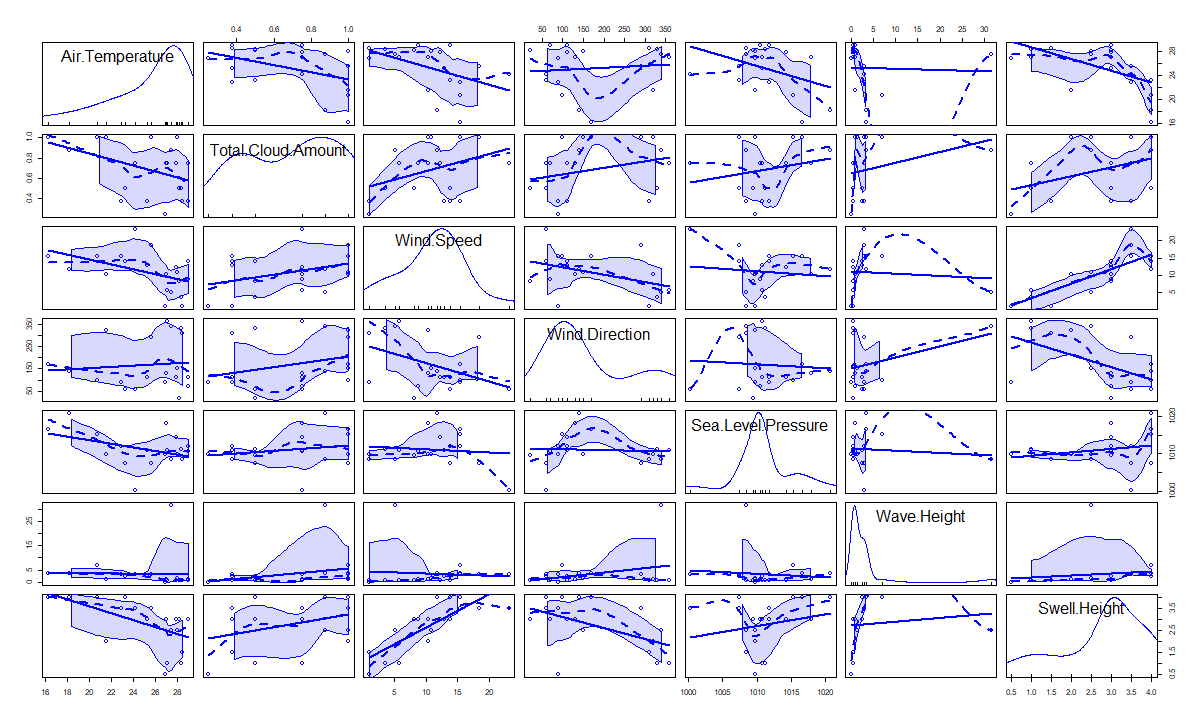
\includegraphics[scale = 0.25]{volume/forecastVarsUnfix.png}
    \caption{Scatterplot Matrix of Main Regressors}
    \label{fig:SPMUnifx}
\end{figure}

As such, there are two major outliers: one in Wave Height at an observed value of $\sim 31.5$ and one in Wind Speed at an observed value of $\sim 46.2$. Removing these values gives the resulting scatterplot matrix:

\begin{figure}[h]
    \centering
    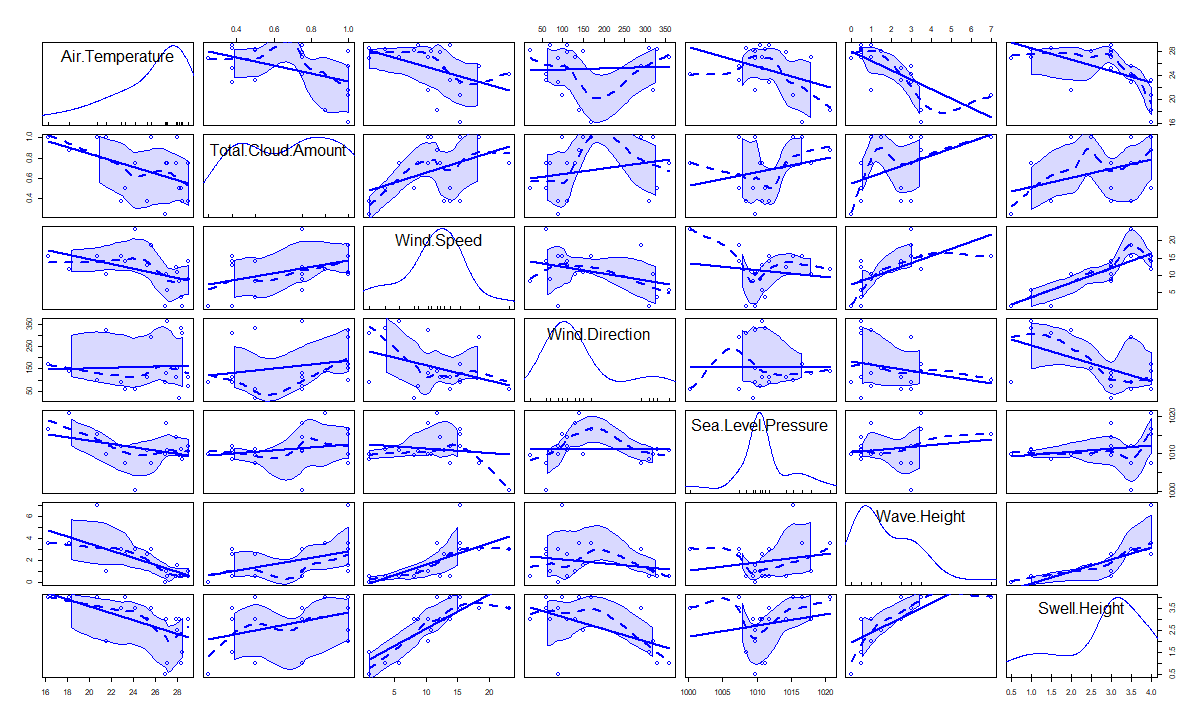
\includegraphics[scale = 0.24]{volume/forecastVarsOutRemoved.png}
    \caption{Scatterplot Matrix of Main Regressors (2 Outliers Removed)}
    \label{fig:SPMFixed}
\end{figure}

\newpage

\subsection{Fitting Linear Models}

After removing these outliers, we create linear models to predict the 7 main regressors from the scatterplot matrix as well as precipitation likelihood. As such, we will generate an n-day forecast using the following algorithmic approach:

\begin{enumerate}
    \item Create a linear model for each of the 8 main regressors using all non-omitted non-NA observations.
    
    \item Use the most recent observation (initially January 31st) as well as the corresponding daily Latitude and Longitude values as our initial input to the mean function of the regressor models.

    \item Generate the next day values for each of the 8 main regressors using the most recent day observation values as inputs to the mean functions. Store these values in the succeeding column.

    \item Repeat steps 2 and 3 n-times to get an n-day forecast prediction.
    
\end{enumerate}

\subsubsection{Reasoning Behind The Models}

For each regressor, we will introduce the model fitted in R, run an overview of the factors contributing to regressor choices in each model \cite{bowditch-2017}, and explain the reasoning behind regressor and response transformations using simplified logic from more advanced atmospheric modeling methods \cite{Jacobson2005-bd}.

\subsubsection*{Sea Level Pressure}

\begin{figure}[h]
    \centering
    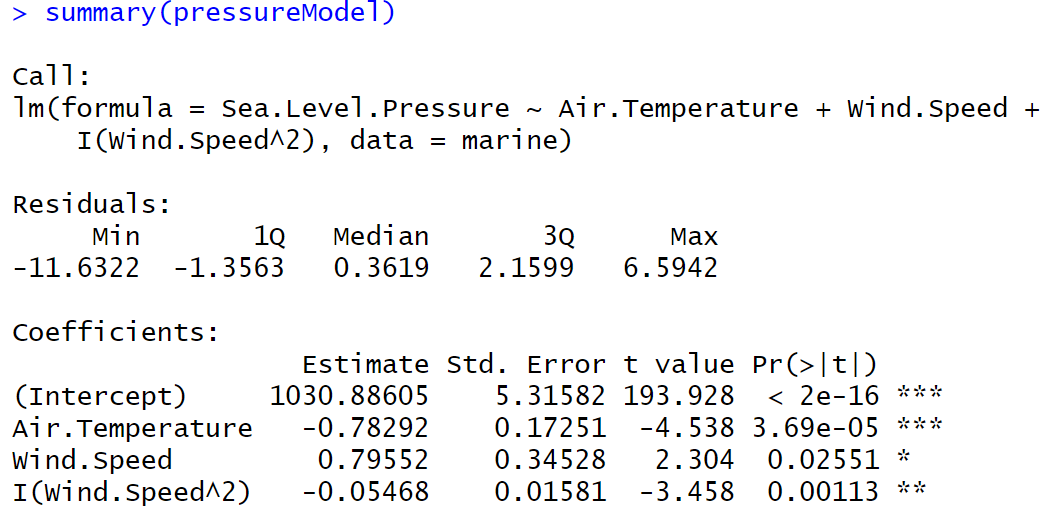
\includegraphics[scale = 0.6]{code snippets/summaryPressure.PNG}
    \caption{Sea Level Air Pressure Model (millibars)}
    \label{fig:PressureModel}
\end{figure}

Air Temperature is included in the model as warmer air has a lower density, creating lower pressure conditions. Wind Speed is included in the model as air flows more aggressively in areas with larger changes in pressure. In addition, the quadratic term for Wind Speed is included to represent the two-dimensional effect of wind and reduce bias towards more extreme wind conditions, typically with wind speeds over 30 meters per second.

\subsubsection*{Air Temperature}

\begin{figure}[h]
    \centering
    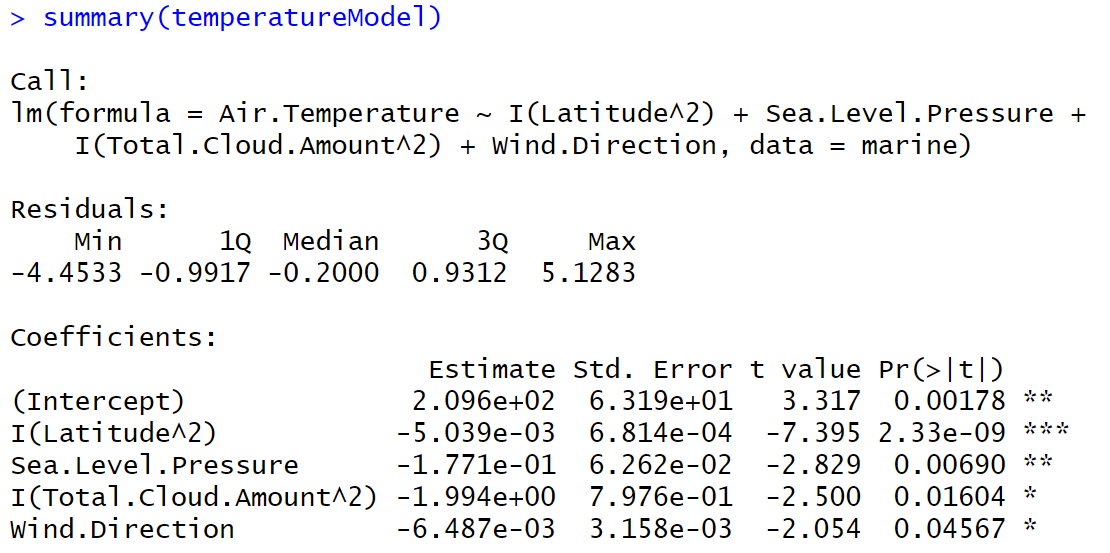
\includegraphics[scale = 0.6]{code snippets/summaryTemperature.PNG}
    \caption{Air Temperature Model (Degrees Celsius)}
    \label{fig:TemperatureModel}
\end{figure}

The quadratic term for Latitude is included in the model as air temperature generally gets colder the farther in magnitude you are from the equator. As such, Sea Level Pressure is included as warmer air is associated with a reduction in air pressure. Total Cloud Amount is included as the sun contributes to heating air particles in the sky. This term is quadratic to account for the two-dimensional coverage clouds have in the sky. Wind Direction is included as depending on geographic location, certain wind directions have stronger average wind speeds that create colder air.

\subsubsection*{Wave Height}

\begin{figure}[h]
    \centering
    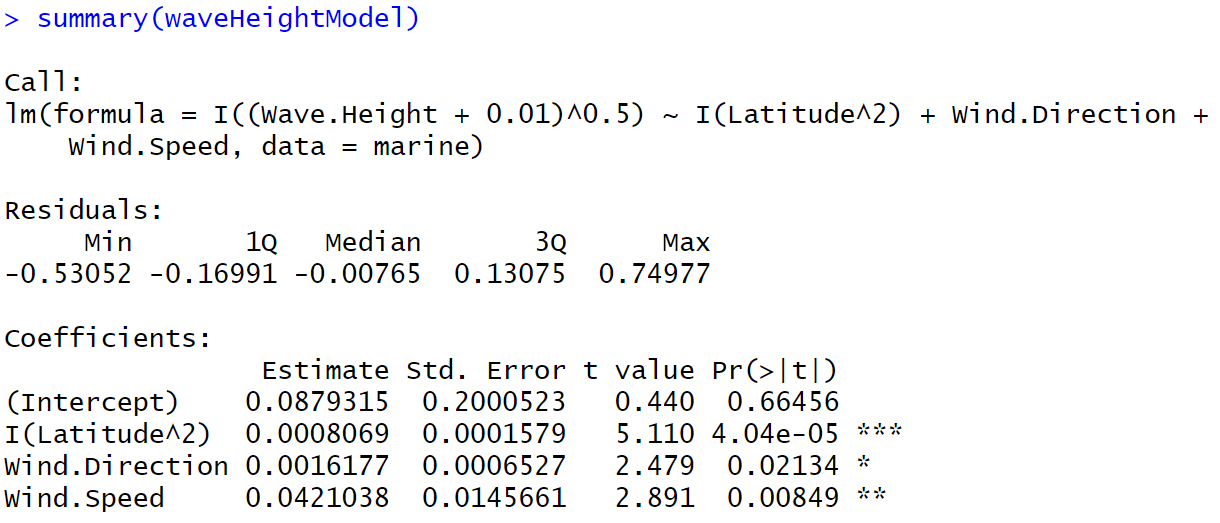
\includegraphics[scale = 0.6]{code snippets/summaryWave.PNG}
    \caption{Wave Height Model (Meters)}
    \label{fig:WaveModel}
\end{figure}

The quadratic term for Latitude is included as waves are typically more aggressive towards the poles due to the Coriolis effect. This effect also directly ties in with the other two regressors for this model: Wind Speed and Wind Direction.

\subsubsection*{Swell Height}

\begin{figure}[h]
    \centering
    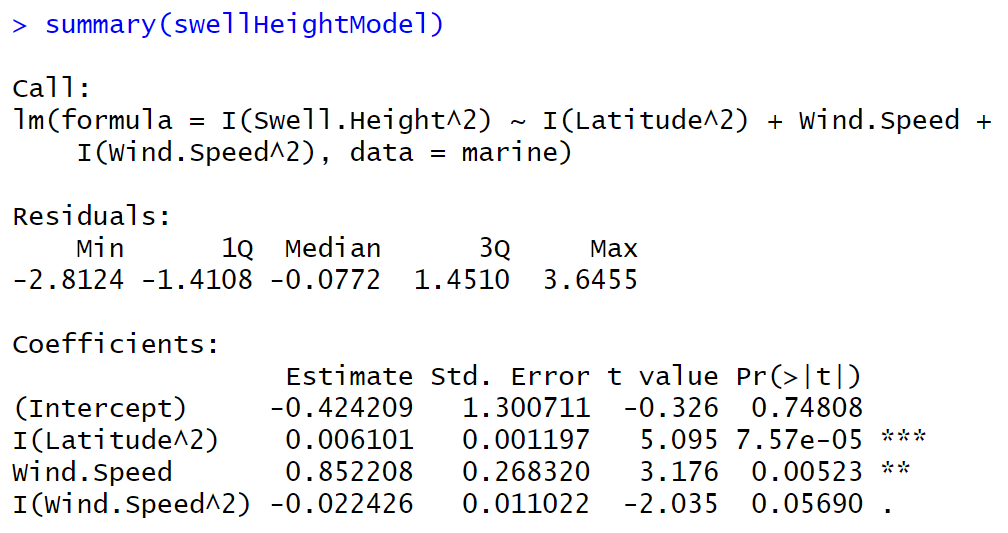
\includegraphics[scale = 0.6]{code snippets/summarySwell.PNG}
    \caption{Swell Height Model (Meters)}
    \label{fig:SwellModel}
\end{figure}

The quadratic term for Latitude is included as swells are more aggressive towards the poles due to the Coriolis effect. Once again, this effect directly ties into the Wind Speed regressor for this model. The quadratic term for Wind Speed is included as swells also concern length, making them more two-dimensional types of observations. Consequentially, this also reduces bias towards more extreme wind conditions, typically with wind speeds over 40 meters per second.

\subsubsection*{Total Cloud Amount}

\begin{figure}[h]
    \centering
    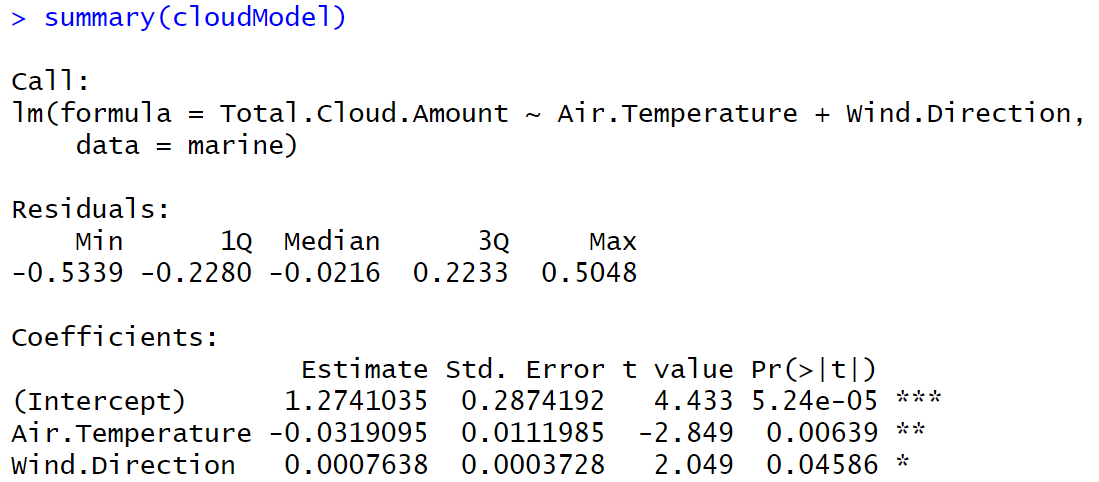
\includegraphics[scale = 0.6]{code snippets/summaryCloud.PNG}
    \caption{Total Cloud Amount (Proportion)}
    \label{fig:CloudModel}
\end{figure}

Air Temperature is included as the reduced air temperature is associated with clouds blocking the sun at times. As such, colder air may signify an increased proportion of cloud coverage. Wind Direction is included due to Hadley Cells, a global atmospheric phenomenon that plays a critical role in the flow of Earth's atmosphere. 

\newpage

\subsubsection*{Wind Direction}

\begin{figure}[h]
    \centering
    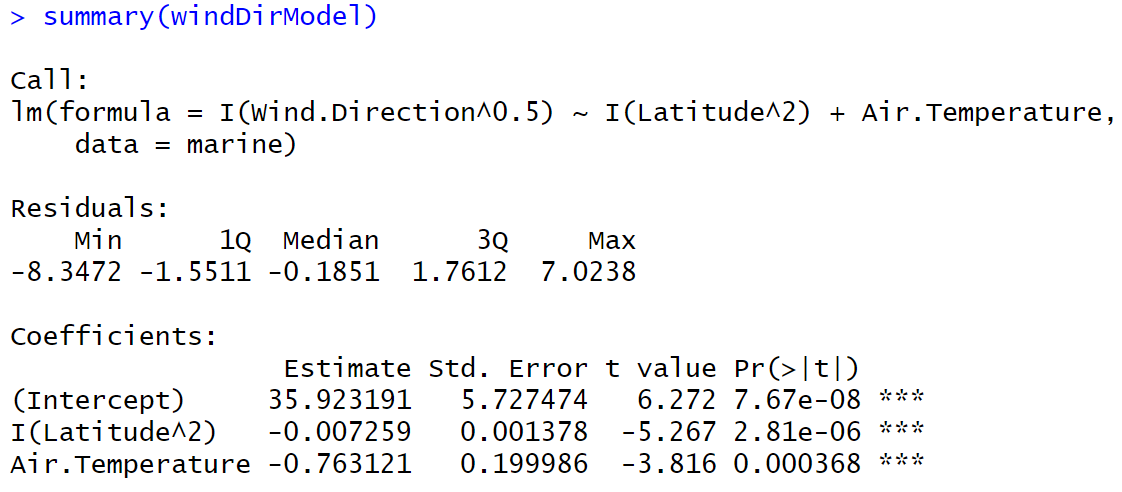
\includegraphics[scale = 0.6]{code snippets/summaryWindDir.PNG}
    \caption{Wind Direction (Degrees Clockwise from North)}
    \label{fig:WindDirectionModel}
\end{figure}

The quadratic term for Latitude is included as the direction of the wind is heavily dependent on the Hadley Cell airflow pattern of Earth's atmosphere. Air Temperature is included as air always travels from cold air to warm air areas due to the pressure difference. While Sea Level Pressure could be included or substituted, Air Temperature captures this change more aggressively in our model.

\subsubsection*{Wind Speed}

\begin{figure}[h]
    \centering
    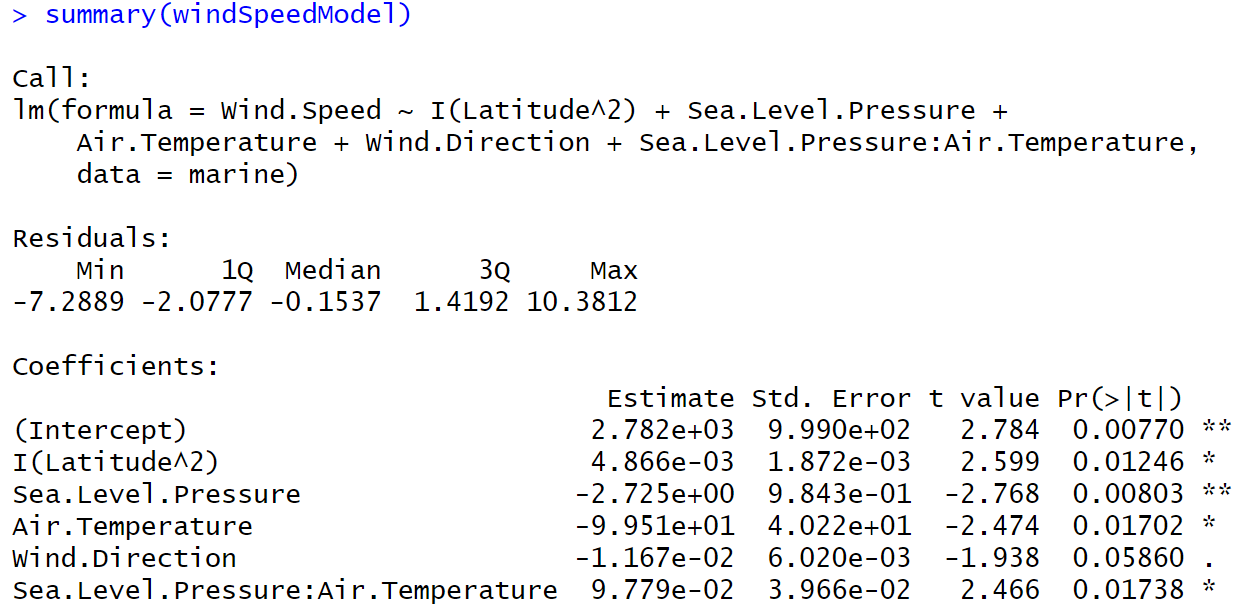
\includegraphics[scale = 0.6]{code snippets/summaryWindSpeed.PNG}
    \caption{Wind Speed Model (Meters per Second)}
    \label{fig:WindSpeedModel}
\end{figure}

The quadratic term for Latitude is included as winds tend to be more aggressive toward the poles. Sea Level Pressure and Air Temperature are included as air wants to flow from colder, higher-pressure areas to warmer, lower-pressure areas. As such, we will include an interaction term between these two regressors to model this interaction. Wind Direction is included as certain directions have higher average Wind Speeds depending on geographic location.

\subsubsection*{Precipitation}

\begin{figure}[h]
    \centering
    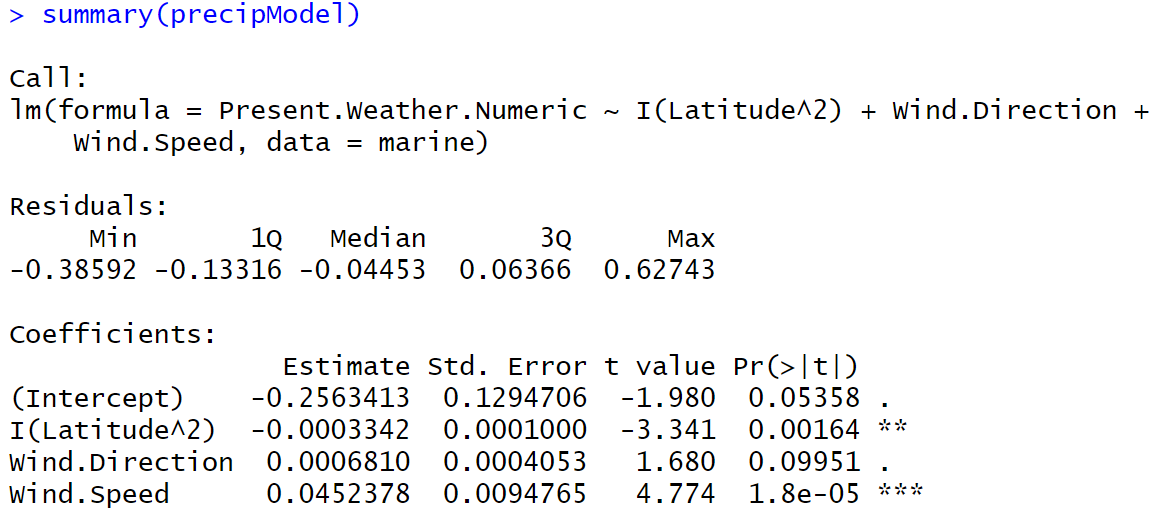
\includegraphics[scale = 0.6]{code snippets/summaryPrecip.PNG}
    \caption{Precipitation Likelihood (Proportion)}
    \label{fig:PrecipitationModel}
\end{figure}

The quadratic term for Latitude is included as precipitation tends to be greatest at and around the Equator. Wind Speed and Direction are included as both are affected by Hadley Cells in the Earth's atmosphere, affecting the flow of air and rain clouds. Sea Level Pressure should be included, but it was deemed to not be statistically significant in our model, evident in the ANOVA test below:

\begin{figure}[h]
    \centering
    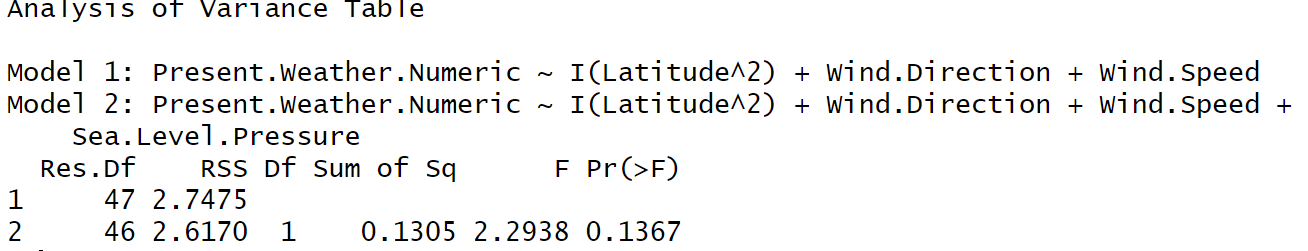
\includegraphics[scale = 0.6]{code snippets/anovaSLPCompare.PNG}
    \caption{ANOVA Table \texttt{AH: + Sea Level Pressure}}
    \label{fig:ANOVASLPComparison}
\end{figure}

\subsubsection{Model Generalization Matrix}

To represent all of these linear models cleanly, we can transform all 8 model predictions into the inverse standard regression form equation below

\begin{equation}
    ((\beta_{0} + \sum_{i=1}^{11} x_i^{\beta_{i}})^{-\beta_{12}}) - \beta_{13}
\end{equation}

and use the row values in the table below (12) for values $\beta_1, ..., \beta_{13}$ for each model. Hypothetical zeros require log transformations, hyphens omit the observation, and commas include multiple powers of a regressor.

\newpage

\begin{figure}[h]
    \centering
    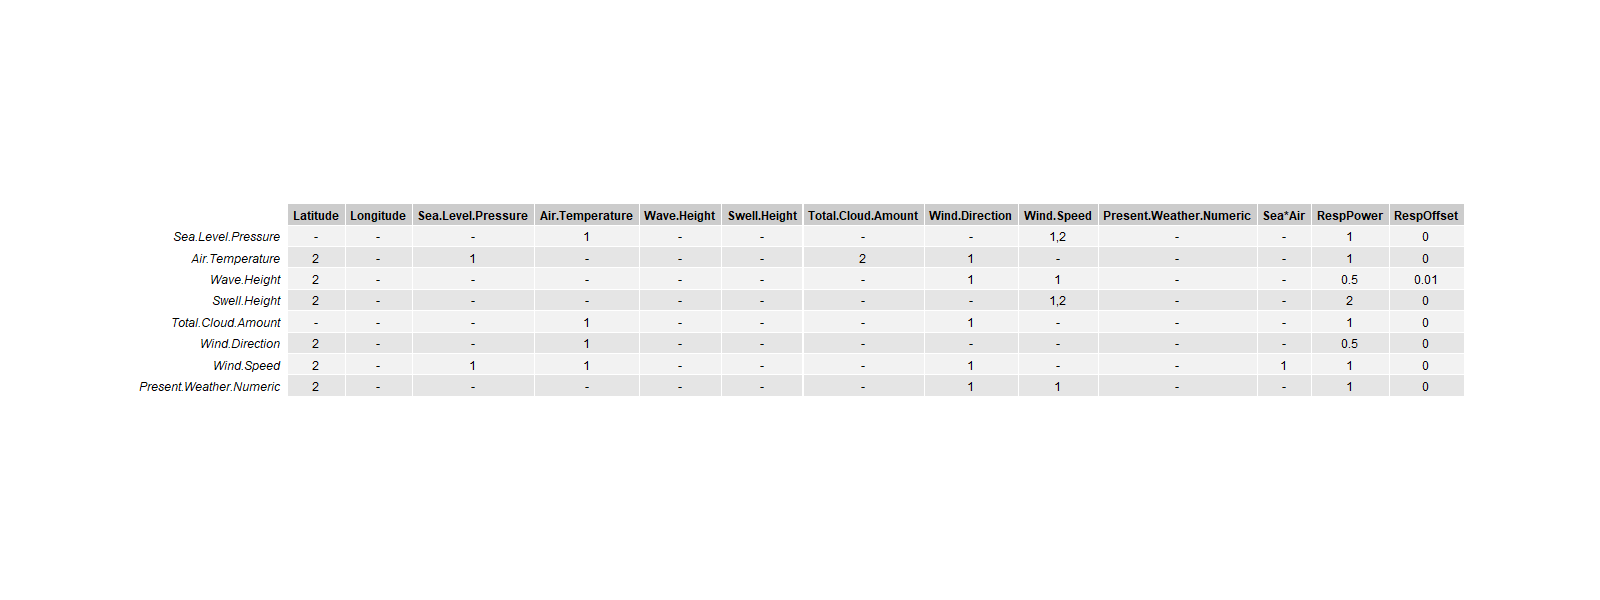
\includegraphics[scale = 0.27]{volume/regressorResponseOffsetMatrix.png}
    \caption{Generalized Power and Offset Matrix for Each Linear Model}
    \label{fig:GenLinModMatrix}
\end{figure}

\subsection{Inverse-Response and Box-Cox Plots}

With our models established, we must justify our response transformations by analyzing the Inverse Response and Box-Cox method plots. As such, these must suggest no other transformation is necessary or can be performed. The IR-BC plots for each of the 8 models are on the next page in Figure 13.

\subsubsection*{Addressing The IR-BC Plots}

Analyzing the IR-BC matrix, six of the eight models require no further transformation as suggested by both a Box-Cox plot containing $\lambda = 1$ in the 95 percent confidence interval for log-likelihood maximization and $\hat \lambda$ estimates in the Inverse Response plots fitting relatively close to the linear transformation $\hat \lambda = 1$. However, we still have two cases to address. For the Present Weather Numeric (Precipitation) variable, these values were artificially generated by converting a previously categorical variable into a numeric one. As such, neither plot provides relevant information for this model. For Sea Level Pressure, it appears that the RSS does not converge to a value for $\hat \lambda$. However, $RSS(\lambda = 1) \approx 265.9$ and $RSS(\lambda = 10) \approx 263.3$. Because $RSS(1)$ and $RSS(10)$ are quite close, it is reasonable to assume that no further transformation is needed, even in the absence of convergence in the Box-Cox log-likelihood maximization.

\newpage

\begin{figure}[h]
    \centering
    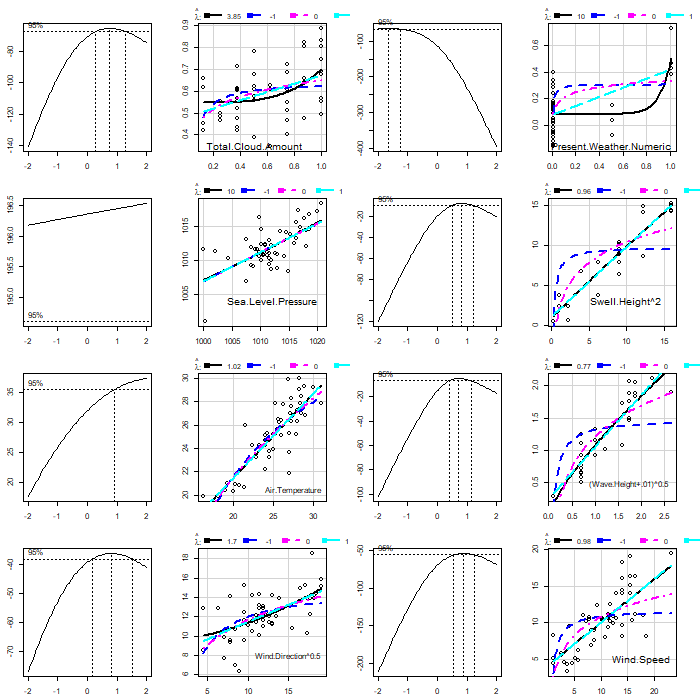
\includegraphics[scale = 0.45]{volume/IRBC_Matrix.png}
    \caption{Inverse Response and Box-Cox Matrix}
    \label{fig:IRBC}
\end{figure}

With our statistical methods and linear models established and verified, we have the framework to create maritime weather forecasts.

\section{Simulating Forecasts}

To put these models in action, we will perform two forecast demonstrations starting at coordinates $(6.1, 94.6)$. These demonstrations will involve a realistic simulation of traveling to Mayabunder, India $(12.9, 92.9)$ over 5 days and an unrealistic simulation of traveling to Augusta, Western Australia \\ $(-34.3, 115.2)$ over 5 days. The red line on the world map graphs indicates the initial path of the vessel with buoy D5GN6 while the blue dots represent the daily Latitude and Longitude values to input for future weather forecasts. As such, the path maps and forecast tables are generated below.

\newpage

\subsection*{Initial Path (Jan 12 to Jan 31)}

\begin{figure}[h]
    \centering
    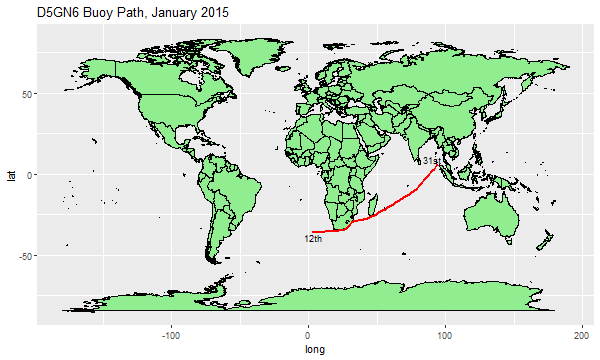
\includegraphics[scale = 0.45]{volume/Buoy_Path_D5GN6.png}
    \caption{Buoy Path from original data, Jan 12th to Jan 31st}
    \label{fig:initPath}
\end{figure}

\subsection{Simulation 1: Mayabunder, India}

\subsubsection*{5-Day Path Visualization}

\begin{figure}[h]
    \centering
    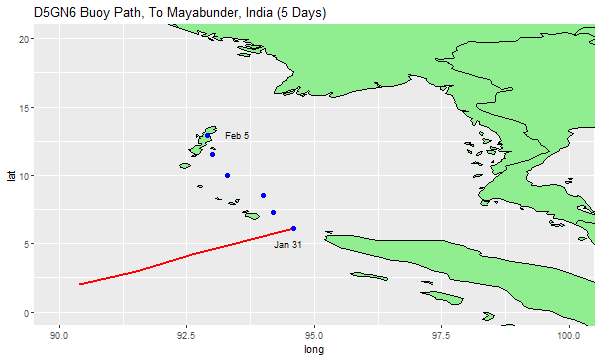
\includegraphics[scale = 0.45]{volume/mayabunderPath.PNG}
    \caption{Hypothetical 5-Day Path to Mayabunder, India}
    \label{fig:mayaPath}
\end{figure}

\newpage

\subsubsection*{5-Day Weather Forecast Table}

\begin{figure}[h]
    \centering
    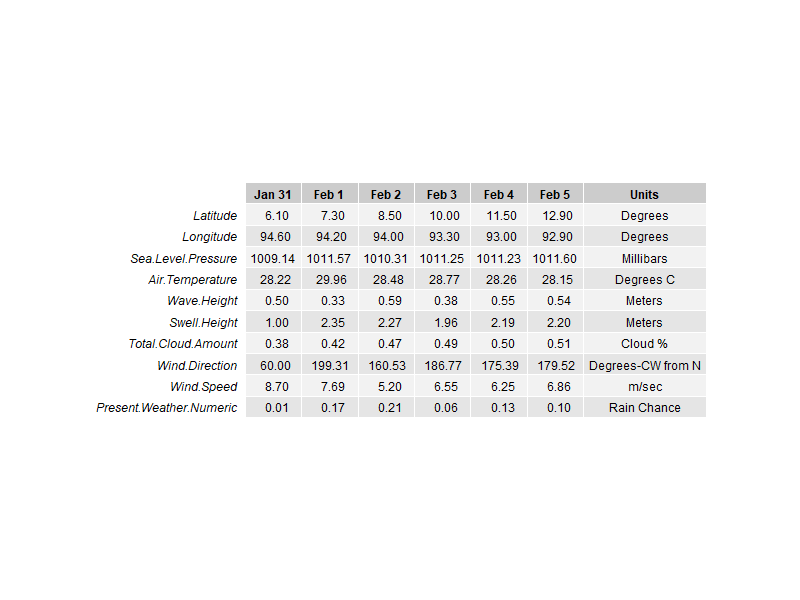
\includegraphics[scale = 0.35]{volume/mayabunderForecastData.png}
    \caption{5-Day Maritime Weather Forecast to Mayabunder, India}
    \label{fig:mayaData}
\end{figure}

\subsection{Simulation 2: Augusta, W. Australia}

\subsubsection*{5-Day Path Visualization}

\begin{figure}[h]
    \centering
    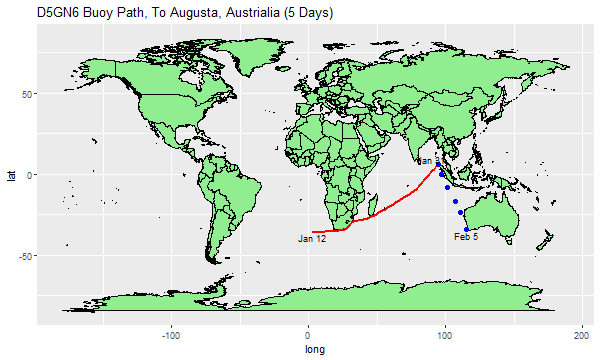
\includegraphics[scale = 0.4]{volume/augustaPath.png}
    \caption{Hypothetical 5-Day Path to Augusta, W. Australia}
    \label{fig:augustaPath}
\end{figure}

\newpage

\subsubsection*{5-Day Weather Forecast Table}

\begin{figure}[h]
    \centering
    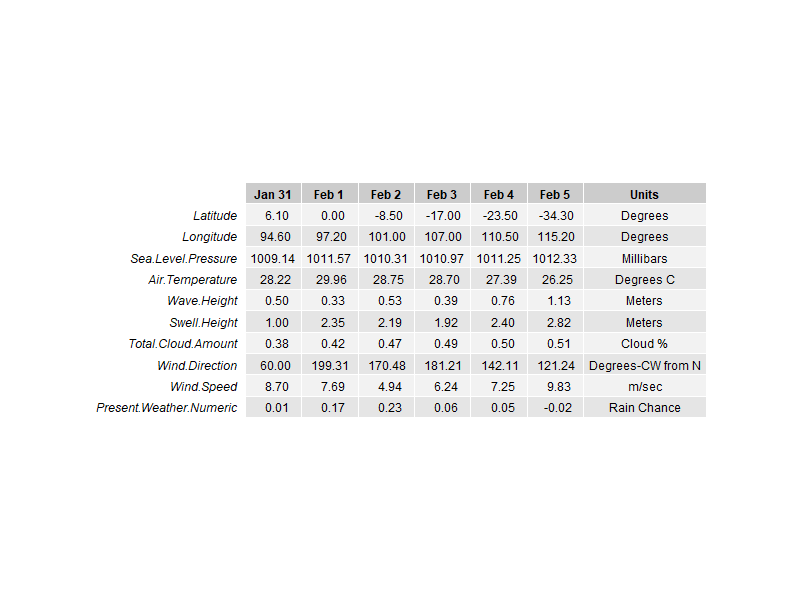
\includegraphics[scale = 0.35]{volume/augustaForecastData.png}
    \caption{5-Day Maritime Weather Forecast to Augusta, W. Australia}
    \label{fig:augustaData}
\end{figure}

\subsection{Strengths and Weaknesses of Forecast}

Comparing the generated maritime to our original data, three main strengths exist. First, our forecasts generated prediction values that are both realistic for the time of year and relatively responsive to sudden changes in Latitude as evident in the Augusta forecast. Second, these forecasts are extremely simple to interpret, especially in comparison to the original observations. Third, the forecast generation is relatively powerful compared to the relatively high-dimension, low-observation characteristics of the original data. Despite these strengths, there are also two major weaknesses in the forecast. First, the predictions generated for each daily weather column depend on the previous day's observations. As such, there will always be some amount of underlying colinearity between the values in each day column. Second, the forecast algorithm tends to be sufficient for roughly 7-14 iterations (days), representable of a real-life weather forecast. Beyond this time frame, some of the weather values may become unstable, trend towards undefined values like \texttt{NaN} and $\infty$, or become uninterpretable. Even in our shorter 5-day simulation to Augusta, the Precipitation Chance on February 5th generated a negative probability.

\section{Conclusion}

In this paper, we analyzed maritime weather measurements from the NOAA, transformed these measurements for exploratory data analysis and modeling, created linear models based on maritime meteorological theory, transformed these models into a weather forecasting algorithm, and analyzed the major strengths and weaknesses behind our forecasting process. As such, there are several actions one could take for further data exploration and fitting. Some of these include applying more advanced regression or machine learning models, using bootstraps to increase the number and power of observations, and applying deeper meteorological and atmospheric theory to fine-tune the model. It is worth noting that some R packages exist specialized specifically for weather analysis and forecasting. As such, the proper application of relevant packages would fit a more accurate and cleaner model than what was created here. However, using R packages was not the objective of this project. Instead, we applied regression modeling techniques, statistical testing, and meteorological theory to create our own weather forecasting model from scratch.

\newpage

%References%

\bibliographystyle{plain}
\bibliography{references}

\end{document}
